% Compile from the repository root; requires graphicx and amsmath.
% These summaries supplement the existing detailed figures.
\begin{figure}[!htbp]
  \centering
  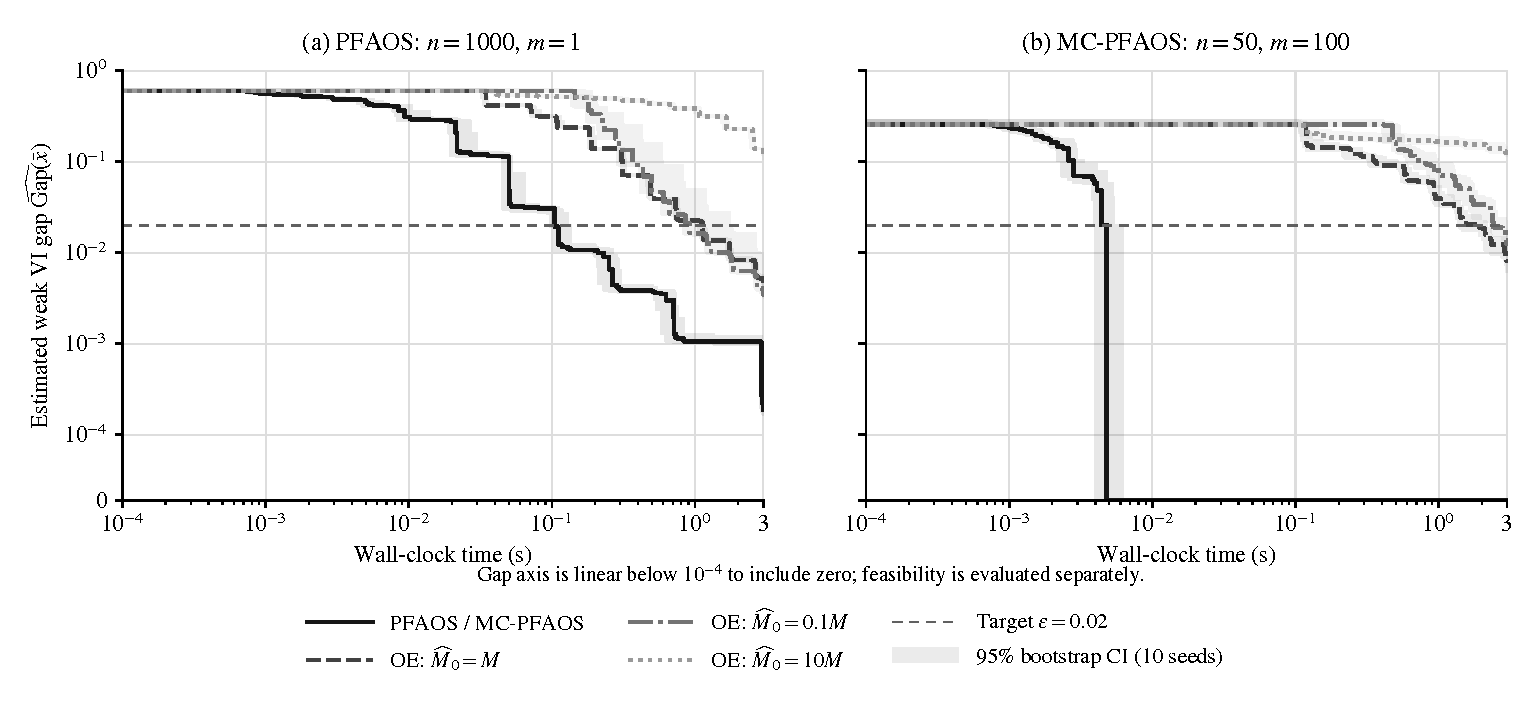
\includegraphics[width=\linewidth]{results/figures/summary_gap.pdf}
  \caption{Estimated weak VI gap against wall-clock time for
  (a) PFAOS at $n=1000$, $m=1$, and (b) MC-PFAOS at $n=50$, $m=100$.
  Projected OE is initialized with $\widehat M_0\in\{M,0.1M,10M\}$,
  where $M=\|B\|_2$; no constraint-smoothness estimate is required.
  Curves show medians over ten seeds, and shaded bands are pointwise
  95\% percentile-bootstrap confidence intervals for the median, using
  2000 resamples of complete seed trajectories. Each seed contributes its
  most recent saved checkpoint, with its supplied initializer available
  at time zero and its final checkpoint retained through the common
  three-second horizon. No interpolation or running minimum is applied.
  The time axis is logarithmic; the gap axis is logarithmic above
  $10^{-4}$ and linear below it to display zero estimates.
  The dashed reference is $0.02$. Gap estimates are numerical primal-objective
  values, not certified upper bounds. A zero gap alone does not imply
  feasibility; joint target attainment is shown in Figure~\ref{fig:summary_error}.}
  \label{fig:summary_gap}
\end{figure}

\begin{figure}[!htbp]
  \centering
  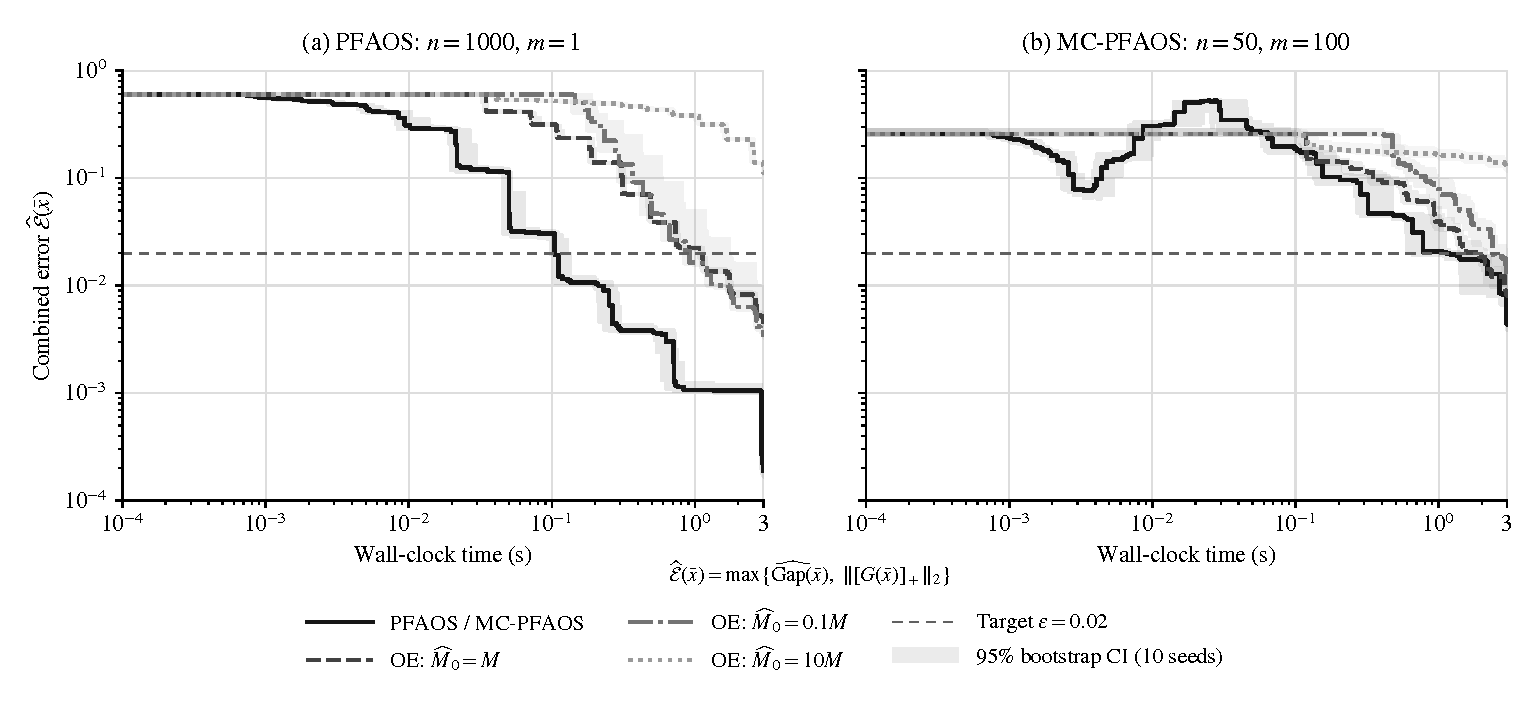
\includegraphics[width=\linewidth]{results/figures/summary_residual.pdf}
  \caption{Combined numerical error
  $\widehat{\mathcal E}(\bar x)=\max\{\widehat{\operatorname{Gap}}(\bar x),
  \|[G(\bar x)]_+\|_2\}$ for the same instances and runs as in
  Figure~\ref{fig:summary_gap}. Both axes are logarithmic.
  Medians and pointwise 95\% bootstrap confidence intervals are computed
  from the per-seed combined error, rather than by combining separate
  median gaps and violations. The dashed reference is the common numerical
  accuracy target $\varepsilon=0.02$.}
  \label{fig:summary_error}
\end{figure}
